%\begin{frame}
%	\frametitle{attacco semplice: Forking}
%	
%\end{frame}
% ----------------------------------------------------------------------------------------------------------------------------
\begin{frame}
	\frametitle{caso di studio: Karame [2012]}

	tipologia transazione 
	\begin{itemize}
	  \item \textit{lenta, e.g.} acquisto ticket eventi
	  		\newline $ \Rightarrow $ sicurezza offerta dal mining
	  \item \textit{{\color{blue}veloce}, e.g.} pagamento in negozio
	  		\newline $ \Rightarrow $ Karame: $\exists $ possibilità di double spending
	  		% negli attuali client, e ci sarebbero comunque se venissero seguite le sole
	  		% precauzioni suggerite prima di questo paper
	  		\begin{itemize}
	  			\item tempi scambio [s] $\ll$ tempi validazione [min]
	  			\item Bitcoin segue tecnica dello struzzo %SAY clients non tenuti ad attendere per transazioni DI POCO CONTO
	  			\item problema limitato in gravità ma non risolto
	  		\end{itemize} 
	\end{itemize}

\end{frame}
% ----------------------------------------------------------------------------------------------------------------------------
\begin{frame}
	\frametitle{caso di studio: Karame [2012]}
	\framesubtitle{garantire validità nel caso \textit{veloce}}

	% SAY curva di probabilità di risoluzione dei blocchi in un certo tempo.
	% 		modellizzata molto bene da una distribuzione geometrica spostata.
	%		quasi un terzo delle transazioni viene confermato in più di dieci minuti !

	\begin{figure}[H]
	 	\begin{center}
			 \begin{tabular}{c @{\hspace{1em}} c}
				 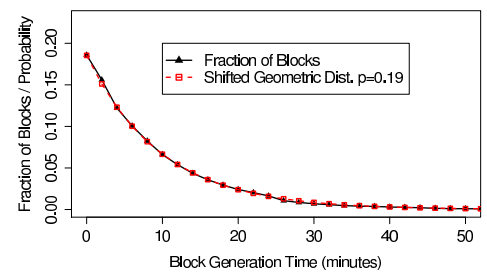
\includegraphics[height=5.5 cm]{images/dspending_1.png}
			 \end{tabular}
		 \end{center}
 	\end{figure}

\end{frame}
% ----------------------------------------------------------------------------------------------------------------------------
\begin{frame}
	\frametitle{caso di studio: Karame [2012]}
	\framesubtitle{ipotesi}

	% SAY curva di probabilità di risoluzione dei blocchi in un certo tempo.
	% 		modellizzata molto bene da una distribuzione geometrica spostata.
	%		quasi un terzo delle transazioni viene confermato in più di dieci minuti !

	\begin{columns}
	 \begin{column}{.45\textwidth}
		hosts
		\begin{itemize}
		  \item $A$ peer disonesto
		  \item $H$ complici di $A$ 
		  \item $V$ vendor onesto
		\end{itemize}
		transazioni
		\begin{itemize}
		  \item $\orange{\mathfrak{T}_V}$: acquisto regolare
		  \item $\orange{\mathfrak{T}_A}$: recupero fraudolento
		\end{itemize}
	\end{column}
	
	\begin{column}{.65\textwidth}
		ipotesi
		\begin{itemize}
		  \item $A$ conosce indirizzo IP di $V$
		  \item capacità di calcolo di $A$ trascurabile % %SAY a differenza della base comune agli attacchi di tipo lento
		  %SAY cioè diretta a indirizzi controllati da A
		  \item $\orange{\mathfrak{I}_V^{in}} = \orange{\mathfrak{I}_A^{in}} \in A$ 
		  \item $ V \ni\, \orange{\mathfrak{I}_V^{out}} \neq \orange{\mathfrak{I}_A^{out}} \in A$
		  \item implementazioni clients: \textit{plain vanilla} %SAY non utilizzate particolari contromisure
	 	\end{itemize}
 	\end{column}
 	\end{columns}

\end{frame}
% ----------------------------------------------------------------------------------------------------------------------------
\begin{frame}
	\frametitle{caso di studio: Karame [2012]}
	\framesubtitle{idea di massima}
 	
 	\begin{columns}
	 \begin{column}{.61\textwidth}
		\begin{itemize}	 
		  	\item $\orange{\mathfrak{T}_V}, \orange{\mathfrak{T}_A}$ inviate contemporaneamente
		  		\newline  $\;\;\Rightarrow $ incluse nello stesso pool %SAY ragionevole inclusione!
	  		\item se $\orange{\mathfrak{T}},\,\orange{\mathfrak{T^\prime}}$ condividono inputs 
	  			\newline $\;\;\Rightarrow $ non ammesse nello stesso pool
	  		\item inclusa solo la prima $\orange{\mathfrak{T}}$ ad arrivare
	  	\end{itemize}
	  	$\;\;\;\;\;\;\;\;\Rightarrow$
	  	\begin{itemize}
	  		\item $\orange{\mathfrak{T}_A}$ da validare rapidamente
	  		\item $\orange{\mathfrak{T}_V}$ sarà smentita dalla rete %SAY ma il vendor si affiderà ad essa intanto
		\end{itemize}
	 \end{column}
	
	 \begin{column}{.6\textwidth}
	 	\begin{figure}[H]
	 	\begin{center}
			 \begin{tabular}{c @{\hspace{1em}} c}
				 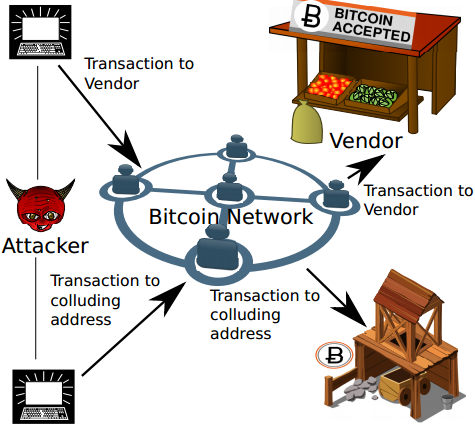
\includegraphics[height=5.5 cm]{images/dspending_2.png}
			 \end{tabular}
		 \end{center}
 		\end{figure}
	 \end{column}
	\end{columns}


% attack can succeed if V receives TRV ,and
% the majority of the peers in the network receive TRA so that TRA is more likely to be included in a subsequent block

\end{frame}
% ----------------------------------------------------------------------------------------------------------------------------
\begin{frame}
	\frametitle{caso di studio: Karame [2012]}
	\framesubtitle{$\mathbf{1^a}$ \textbf{condizione}: connessione diretta}
	
	\fbox{$V$\,riceve prima\,$\orange{\mathfrak{T}_V}$\,di\,$\orange{\mathfrak{T}_A}$}
		\, oppure\,$V$\,includerebbe prima\,$\orange{\mathfrak{T}_A}$\,nel pool
	
	\begin{columns}
		\begin{column}{.5\textwidth}
			\begin{itemize}
			  \item $A$ conosce IP di $V$
			  \item client accetta sempre nuove connessioni < 125 max
			  \item $A$ comunica con $H$
				\begin{itemize}
					\item senza latenza
					\item privatamente    
				\end{itemize}
			  \item $H$ non comunica con $V$
			  \item $A$ invia
				\begin{enumerate}
				  \item $\orange{\mathfrak{T}_V}$ a $V$
				  \item $\orange{\mathfrak{T}_A}$ a $H$
				\end{enumerate} %SAY il tempo a cui V riceve T_V è inferiore a quello in cui riceve T_A
			\end{itemize}
			 $\;\;\;\;\Rightarrow \orange{t_V^V} < \orange{t_V^A}$
		\end{column}
		
		\begin{column}{.60\textwidth}
			\begin{figure}[H]
		 	\begin{center}
				 \begin{tabular}{c @{\hspace{1em}} c}
					 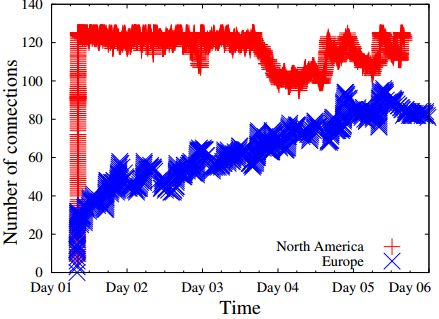
\includegraphics[height=4.75 cm]{images/dspending_3.png}
				 \end{tabular}
			 \end{center}
				\caption{analisi del momento propizio}
	 		\end{figure}
		\end{column}
	\end{columns}		  
\end{frame}
% ----------------------------------------------------------------------------------------------------------------------------
\begin{frame}
	\frametitle{caso di studio: Karame [2012]}
	\framesubtitle{$\mathbf{2^a}$ \textbf{condizione}: diffusione manipolata}
	
	\fbox{$\orange{\mathfrak{T}_A}$ inclusa in blockchain (\textit{i.e.} confermata) prima di
	$\orange{\mathfrak{T}_V}$} \vspace{0.1cm} \newline oppure $\orange{\mathfrak{T}_A}$ non potrebbe seguire $\orange{\mathfrak{T}_V}$ in blockchain
	  		
	\begin{itemize}
	  \item $H$,\,$V$ probabilmente lontani $\;\;\Rightarrow \orange{\mathfrak{T}_A}, \orange{\mathfrak{T}_V}$ broadcastate finchè 
  			$ \left \{
					  \begin{array}{lcr}
					    \text{ogni peer include}\;\orange{\mathfrak{T}_A}\:\dot{\vee}\:\orange{\mathfrak{T}_V}\;\text{in proprio pool}\\
					    \orange{\mathfrak{T}_A}\:\vee\:\orange{\mathfrak{T}_V}\;\text{è confermata}
					  \end{array}
					\right. $ 
	  \item $\Pr[\orange{\tau_A} < \orange{\tau_V}] \propto \sfrac{\orange{\eta_A}}{\orange{\eta_V}}$ governabile in due modi
	  		% TAU: tempo di inclusione in Blockchain
	  		% ETA: #peers che hanno incluso la transazione nel proprio pool
  		\begin{itemize}
  			\item invio di $\orange{\mathfrak{T}_A}$ precede invio di $\orange{\mathfrak{T}_V}$ 
  			\item $H$ aiutano $A$ diffondendo $\orange{\mathfrak{T}_A}$ e filtrando $\orange{\mathfrak{T}_V}$ 
  		\end{itemize}
	  \item ulteriori ipotesi
	  	\begin{itemize}
	  	  	\item $\exists$ istante ove $\orange{\mathfrak{T}_A},\,\orange{\mathfrak{T}_V}$ convivono
	  	  	\item $\forall\,\orange{\varepsilon}\;\mathrm{p.a.p.},\;\;\;
	  	  			\Pr[\orange{\tau_A}\sim\mathrm{secs}]\cup\Pr[\orange{\tau_V}\sim\mathrm{secs}]<\orange{\varepsilon}$ 
	  	  		%SAY HP: non è possibile che nessuna delle due sia confermata in pochi secondi dall'invio
  			\item $\orange{\eta_A},\,\orange{\eta_V}$ non scambiano blocchi risolti $\Rightarrow \orange{\tau_A},\,\orange{\tau_V}$ indipendenti
  			%the time required by peers that are mining in favor of TRV to generate a new block
  			%is independent of that required by the peers that are mining in favor of TRA 
	  	\end{itemize}
	\end{itemize}
	
	%probability of successful block generation in each δt can be modeled as a Bernoulli trial with success probability η p
	%	η is the number of peers  
	%	p the success probability of a peer in generating a block within δt

\end{frame}
% ----------------------------------------------------------------------------------------------------------------------------
\begin{frame}
	\frametitle{caso di studio: Karame [2012]}
	\framesubtitle{probabilità di successo}

	$\Pr[\text{successo in un tempo}\;\orange{\delta t}] \sim \mathrm{Bernoulli}(\orange{\eta},\,\orange{p})$
	\begin{itemize}
	  \item $\orange{\eta}=$ numero di peers coinvolti
	  \item $\orange{p}=\Pr[\,\text{peer generi un }\:\mathfrak{B}\:\text{in}\;{\delta t}\,]$ 
	\end{itemize}

	\begin{figure}[H]
	 	\begin{center}
			 \begin{tabular}{c @{\hspace{1em}} c}
				 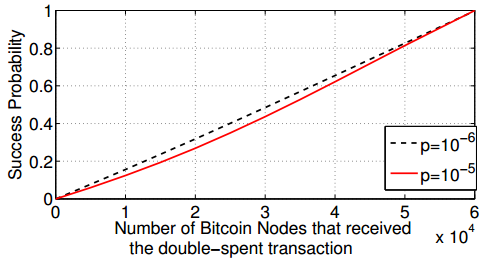
\includegraphics[height=4.5 cm]{images/dspending_4.png}
			 \end{tabular}
		 \end{center}
		 \caption{$\Pr[\mathrm{successo}\;|\;\delta t=10s,\;\eta=6\cdot10^4]$}
 	\end{figure}

 	%SAY dal numero di nodi che hanno ricevuto la doppia transazione, si può dare una stima della probabilità che qualche pool
 	% 	riesca a risolverla e a propagarla

\end{frame}